\renewcommand{\hatabstractname}{\whatshatabstractname}


\typein[\typeinversion]{a.Version with numbers.You can use command``noa''``BA''}
\typein[\whatshatabstractname]{b.type in the hat abstract name,E.G.you can use command``nob''``nobhat''``BB''}
\typein[\hatabstractcontents]{c.Typein abstract contents.E.G.You can use command``noc''``noprint''``origintal''``BC''``noticewave''}
\typein[\typeinincludefiles]{d.Type in what files else you would like to load here.E.G.:abstract2,appendix,appendix2.You can use command``nod''``BD''}
\typein[\typeinauthor]{e.Author's name.E.G.You can use command``noe''``noehat''``BE''}
\typein[\typeindate]{f.Date.E.G.You can use command``nof''``nofhat''``BF''}







\includeonly{main,\typeinincludefiles}


\title{语文笔记}
%\title{语文笔记 Ver \typeinversion}
\author{\typeinauthor}
\date{\typeindate}
\begin{document}
\pagenumbering{alph}
\maketitle
\begin{hatabstract}
\hatabstractcontents
\end{hatabstract}
% # -*- coding: utf-8 -*-
\typeout{now loading abstract2.tex}
\begin{abstract}
\begin{enumerate}
\item 一套徐正华老师的上课笔记
\item 由HAWX AT TEAM整理
\item 徐正华:
\begin{itemize}
\item 未知年进入立达中学,立达中学变态老师之首
\item 历届立达初三理科班班主任兼语文老师
\item 以讲作文著名
\item 超级色
\item 历届立达初三理科班语文在黄浦区排名第一
\item 曾经亲手解散江蔚峰老师建立的9班附属疯人院
\item 21世纪的火星人
\end{itemize}
\item 请查询此蓝本计划BLUEPRINT-ywjtffdq
\end{enumerate}
\begin{center}

\includegraphics[width=4.5cm]{info.png}
\end{center}
\end{abstract}
\newpage
\begin{center}
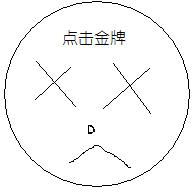
\includegraphics[width=4.6cm]{readme}
\end{center}
\begin{verbatim}
click gold medal
初中语文——解题方法大全
主编:徐正华
“做人做不好,作文怎么可能写得好”
图书在版编目(CIP)数据
初中语文解题方法大全/徐正华主编——上海:猥亵出版社
ISBNXXX-X-XXXX-XXXX-X
Ⅰ初……Ⅱ徐……Ⅲ语文课-初中-解题
ⅣXZ.H438
中国版本图书馆CIP数据检字(2012)第XXXXXX号
猥亵男出版集团·上海猥亵出版社出版发行
(https://sites.google.com/site/zdsxxz)
猥亵男不负责印刷
&经销
2012年12月22日第-1版 上海version3 No印刷
开本:000*0000毫米  1/0 印张00.000
字数:X字 印数000000-000000
定价:-1元
\end{verbatim}\label{abstractinformal} 

% # -*- coding: utf-8 -*-
\typeout{now loading main.tex}
\pagenumbering{roman}
\tableofcontents
\label{contents}
\newpage
\pagenumbering{arabic}

\section{现代文知识(概念)}

\hatsubsection{句子根据语气分:}
陈述句、疑问句、祈使句(请求、命令、期望、劝阻、催促)感叹句

\hatsubsection{语言表达方式:}
叙述、描写、议论、抒情、说明

\hatsubsection[\hatx{1}{2011-05-24}]{修辞方法:}
设问(问号)、反问(问号)、排比(三者)、对比、比喻、拟人、夸张(夸大或缩小)、引用

\hatsubsection[\hatb{41}{1}{2011-05-24}]{描写(细分):}
\begin{compactdesc}
\item[人物:]肖像(外貌、神态)、动作、语言、心理;
\item[环境:]自然、社会
\end{compactdesc}
\hatsubsection{记叙顺序:}
顺叙、倒叙、插叙(中间的段落)

\hatsubsection{说明顺序:}
时间、空间、逻辑

\hatsubsection[\hatb{41}{1}{2011-06-14}]{说明方法:}
列数字、举例子、作比较、列图表;下定义、引资料、分类别、打比方

\hatsubsection[\hatb{41}{1}{2011-05-24}]{论据的种类:}
\begin{compactdesc}
\item [事实论据]有代表性的确凿的事例,历史史实,统计数字等(事例史实以及数据)
\item [理论论据]经典著作,权威性言论,名人名言,警句,言语,俗语,自然科学的原理、定律、公式等
\end{compactdesc}

\hatsubsection[\hatx{1}{2011-06-14}]{论证方法:}
例证法(举例论证法)、引证法(引用论证法)、对比论证、比喻论证、类比论证

\hatsubsection{论证结构(思路结构):}
总分式、并列式、层进式、对照式

\hatsubsection[\hatx{1}{2011-06-14}]{小说三要素:}
\begin{compactdesc}
\item[小说]小说的中心,反映文章主题
\item[环境]分为自然环境、社会环境
\item[故事情节]故事的开端、发展、高潮、结局
\end{compactdesc}

\hatsubsection[\hatx{1}{2011-08-04}]{第二人称:}
能体现一种亲切感、亲密感,更便于作者的抒情

\section{现代文综合知识(方法)}

\hatsubsection{词的感情色彩:}
褒义贬用(讽刺了\ldots{}\ldots{});贬义褒用(使语言幽默生动)

\hatsubsection[\hatb{6}{2}{2011-06-13}]{词序(词或词组能否互换):}
\begin{asparaenum}[(1)]
\item 逻辑关系(大多数):\ldots{}\ldots{}(前者)是\ldots{}\ldots{}(后者)的前提(或\ldots{}\ldots{}(后者)在\ldots{}\ldots{}(前者)的基础上才能形成,或先有(前者)\ldots{}\ldots{},才有\ldots{}\ldots{}(后者));符合其发生、发展逻辑顺序(或符合人们认识事物的客观规律)
\item 强调作用:突出了\ldots{}\ldots{}(极少)
\end{asparaenum}

\hatsubsection[\hatm{NI}{1}{2011-06-14}]{选择词语:}
一种是选择能表现人物思想性格的词语(围绕``表现人物的思想性格''来回答);另一种按照``辨析近义词''的方法进行

\hatsubsection[\hatb{41}{1}{2011-05-25}]{句子的含义:}
表层:字面(扣住语境);深层:深刻、含蓄、双关、暗示等

\hatsubsection{句子在文中的作用:}
\begin{asparaenum}[(1)]
\item 句式特点(结合文体):记叙文——铺垫、伏笔、照应、过渡;描写、修辞、设置悬念等;说明文——过渡、照应;说明方法等;议论文——过渡、照应;论据、论证方法等)
\item 表现中心(包括一部分文字的中心)
\end{asparaenum}
(结尾处的作用有内容上:点明中心、深化主题:结构上照应开头、点题等)\par
注意:过渡通常有两种情况:承上启下和引出下文

\hatsubsection[\hatx{1}{2011-08-04}]{选择句子或词语:}
总是为了更好地表达中心、思想感情、人物形象
\hatsubsubsection{选择句子:(哪句句子好)}
依据句式特点进行:修辞句、描写句;哲理句、倒装句(句子成分、分句)(分号后面的少)


\hatsubsection{句序(语句能否互换):}
\begin{asparaenum}[(1)]
\item 过渡作用;
\item 照应作用;
\item 主次关系;
\item 总分关系
\end{asparaenum}

\hatsubsection{填写句子:}
\begin{asparaenum}[(1)]
\item 填写承上启下的过渡句(包括起过渡作用的设问句);
 \item 填写总起句(中心句)
\end{asparaenum}

\hatsubsection{反问句与陈述句谁好:}
\begin{asparaenum}[(1)]
\item 反问句能表达更加强烈语气,强调了\ldots{}\ldots{}(该句要表达的意思):
\item 写出这两句加强(削弱)了\ldots{}\ldots{}语气((1)居多)
\end{asparaenum}

\hatsubsection[\hatx{1}{2011-09-26}]{段序(段与段能否互换):}
\begin{asparaenum}[(1)]
\item 过渡关系(承上启下);
\item 连接关系(与上下段的关系);
\item 总分关系;
\item 照应关系;
\item 递进关系;
\item 主次关系;
\item 时间关系;
\item 空间关系
\end{asparaenum}

\hatsubsection{段落在文中的作用:}
同``5的句子在文中的作用'';记叙文中加考虑是否``插叙''

\hatsubsection{指代:}
往往在它的前面,往往原文中有现成的;\uuline{代入法验证}

\hatsubsection[\hatx{3}{2011-09-26}]{设问(设问句)的作用:}
\begin{compactdesc}
\item[文中]引起读者的注意和思考,使文势有变化,在结构上起过渡(分为承上启下和启下)作用,引出下文(概括)(,突出某些内容),使文章结构紧密,条理清楚。
\item[标题]引起读者的注意和思考,能更好的表现\ldots{}\ldots{}中心;增加读者的阅读兴趣
\end{compactdesc}

\hatsubsection{反问的作用:}
表达更加强烈的语气,更加肯定的意思(要分析)\\

\hatsubsection[\hatb{6}{2}{2011-06-13}]{排比的作用:}
\begin{asparaenum}[(1)]
\item 增强语言气势,强调或突出了\ldots{}\ldots{}(排比句想要表达的意思,即中心):
\item 分别从几个角度描绘(说明、论证)了\ldots{}\ldots{}(较少)
\end{asparaenum}

\hatsubsection{对比的作用:}
将\ldots{}\ldots{}与\ldots{}\ldots{}作对比,突出了\ldots{}\ldots{}

\hatsubsection{比喻(拟人):}
\begin{asparadesc}
\item[记叙文:]生动形象地描写了\ldots{}\ldots{}(内容),从而表现了\ldots{}\ldots{}(中心);\\
\item[说明文:]生动形象地说明了\ldots{}\ldots{}(使说明的内容通俗易懂);\\
\item[议论文:]生动形象地论证了\ldots{}\ldots{}
\end{asparadesc}

\hatsubsection{夸张的作用:}
强调了\ldots{}\ldots{},(有的还要``从而表现了\ldots{}\ldots{}'')

\hatsubsection[\hatx{1}{2011-09-26}]{语言表现力(赏析):}
运用了\ldots{}\ldots{}(特色:\begin{inparaenum}[(1)]\item 修辞手法;\item 描写方法;\item 其它\ldots{}\ldots{}\end{inparaenum})+(具体)生动形象地写出了\ldots{}\ldots{}(如人物的动作、神态、心理活动、景物怎样的特征等)(,为下文的\ldots{}\ldots{}作铺垫)或(,为下文的\ldots{}\ldots{}作对比)+从而表现出(或说明了、论证了)\ldots{}\ldots{}(对表达文章中心起的作用)\par
注:仅在有细节描写时考虑``具体''\\
仅记叙文中考虑``,为下文的\ldots{}\ldots{}作铺垫''\\
``其它''指:褒义贬用/贬义褒用、动词/形容词连用、拟声词、叠词;倒装句、整句和散句等
\hatsubsection{冒号用法:}
\begin{asparaenum}[(1)]
\item 提示下文;
\item 总结上文
\end{asparaenum}

\hatsubsection{引号用法:}
\begin{asparaenum}[(1)]
\item 表示引用;
\item 强调,着重指出;
\item 表示特殊含义(或特定的称谓);
\item 反语,表示讽刺或否定
\end{asparaenum}

\hatsubsection{破折号的用法:}
\begin{asparaenum}[(1)]
\item 补充、解释说明;
\item 意思的转折(话题的转换);
\item 表示意思的递进;
\item 表示语音的延长或停顿、中断
\end{asparaenum}

\hatsubsection[\hatx{1}{2011-09-26}]{省略号用法:}
\begin{asparaenum}[(1)]
\item 表示列举的省略;
\item 表示内容的省略;
\item 表示说话断断续续或含含糊糊、支支吾吾
\item (为了更好表现中心)
\end{asparaenum}

\hatsubsection[\hatx{1}{2011-09-26}]{括号的作用:}
补充说明

\hatsubsection{书名号用法:}
书名、报名、刊名、篇名、剧名等

\hatsubsection[\hatx{1}{2011-09-26}]{思想感情:}
作者的思想感情往往在文章的结尾

\hatsubsection{以下内容未确定:}
\hatsubsubsection{表达特点:}
\hatm{NI}{2011-08-24}\uwave{修辞手法和描写方法}

\hatsubsubsection{表达效果:}
\hatm{NI}{2011-08-24}\uwave{修辞手法和描写方法的作用}

\hatsubsubsection{照应的作用:}
\hatm{NI}{2011-08-24}\uwave{前后照应,(使)结构严谨,表现中心}

\hatsubsubsection{作者的思想感情<记叙文>}
\hatm{基本修补成功,已放入文档}{2011-09-26}\uwave{往往在文章结尾出现}

\hatsubsubsection{安排详略的作用<记叙文>}
\hatm{NI}{2011-09-26}\uwave{为了更好的表现中心}

\hatsubsubsection{议论文语言特点-议论文语言严密性:4.10.1}
\hatm{NI}{\uwave{2011-09-26}}

\section{记叙文}

\hatsubsection[\hatx{1}{2011-09-26}]{记叙文整体感知:}
目标:写了\ldots{}\ldots{}(概括全文的内容);表现了(赞美或揭露了;揭示了哲理)\ldots{}\ldots{}(有时还有表达了\ldots{}\ldots{}思想感情)\par
方法:\begin{asparaenum}[(1)]\item 看题目(中心内容/思想意义);
        \item 圈划出评价人或物的词句;
        \item 划出议论句、抒情句、哲理句(*文中反复出现的也要划出来);
        \item 看开头与结尾(尤其是看(划)结尾部分):
        \item 看内容与细节描写处;
        \item 看题干
\end{asparaenum}

\hatsubsection[\hatx{1}{2011-09-26}]{片段:}
续写:
\begin{asparaenum}[(1)]
\item 要符合原文中的情节的延续,人物的形象
\item 语言风格要保持一致
\item 要能更好的表现中心
\item 照应上文,点题
\end{asparaenum}
写作特点
\begin{asparaenum}
\item 观点(本文的人物(景物)描写很有特色,\ldots{})\\如文中第X段的\ldots{}(例子),生动形象地写出了\ldots{}(概括这段内容),从而表现出\ldots{}(中心)
\end{asparaenum}

\hatsubsection{词语在文中的含义;}
结合语言环境作具体解释;少数结合其在古汉语中的意思

\hatsubsection{是否矛盾:}
``殊途同归'':从两个角度分别叙述,(有时要写明是为了更好地表现中心)

\hatsubsection{概括:}
一般由``谁''+``做了什么''进行表达(但不是字越少越好)

\hatsubsection{``具体表现'':}
在文中可以找到

\hatsubsection{点评语句:}
或从内容(包括中心)方面,或从语言特点上进行

\hatsubsection{顺叙的作用:}
可以使事情的来龙去脉清晰地表现出来

\hatsubsection{倒叙的作用:}
使结构有变化,叙述有波澜,以制造悬念,引人入胜;对比(较少)

\hatsubsection[\hatx{3}{2011-09-26}]{插叙的作用:}
补充交待了\ldots{}\ldots{}(概括这部分内容)(有的有``为下文的\ldots{}\ldots{}作铺垫''或``和下文的\ldots{}\ldots{}作对比'')+更好地表现了\ldots{}\ldots{}(结合``中心''分析)+使文章更充实,内容更生动,主旨更突出(人物形象更鲜明)\par
注:仅在中间段落考虑插叙

\hatsubsection{人物描写的作用:}
刻画其思想品质和性格特征(有时表现人物的思想感情)\par
侧面描写:为正面描写服务,即能更好地刻画人物的形象\\
细节描写:刻画人物思想品质和性格特征\par
方法:生动形象地写出了\ldots{}\ldots{}(内容),从而表现出\ldots{}\ldots{}(中心)

\hatsubsection{补充心理描写:}
常见的有表达``感激、愧疚\ldots{}\ldots{}或矛盾的心理''等;要能连接上下文:不能太短

\hatsubsection[\hatx{2}{2011-07-19}]{环境描写的作用:}
\begin{asparaenum}[(1)]
\item 交代故事发生的时间、地点(或背景)(一般在开头);
\item 渲染\ldots{}\ldots{}气氛,营造\ldots{}\ldots{}氛围,确定\ldots{}\ldots{}基调;
\item 烘托\ldots{}\ldots{}心情(或思想感情);
\item 为下文\ldots{}\ldots{}作铺垫(较少有``与下文\ldots{}\ldots{}相照应''、``与文中\ldots{}\ldots{}作对比'');
\item 推动故事发生的情节(非头尾段);
\item 刻画人物思想性格;
\item 表现主旨,突出文章中心
\end{asparaenum}

\hatsubsection{详写与略写:}
依据``能否更好地表现中心思想''来回答

\hatsubsection{结尾部分的作用:}
结构:\begin{asparaenum}[(1)]\item 照应开头;
        \item 点明标题;\\
内容:\item 突出主旨;
        \item 深化主题(有时还有含蓄生动,耐人寻味,给予读者以想象等)\end{asparaenum}
        (深化主题:通常有两种\begin{inparaenum}[(1)]\item 揭示深刻的哲理\item 其品质(精神)影响到他人。\end{inparaenum})

\hatsubsection[\hatx{1}{2011-09-26}]{标题的含义:}
\begin{asparaenum}[(1)]
\item 浅层(与中心内容有关);(要为后面深层服务)
\item 深层(与思想意义有关)
\end{asparaenum}

\hatsubsection[\hatx{1}{2011-09-26}]{标题的作用:}
\begin{asparaenum}[(1)]
\item 写作特点\\
三种文体都有:``运用比喻的修辞手法''(生动形象地)、``运用设问的修辞手法''(引起读者的阅读与思考,引起读者的阅读兴趣).\\
单记叙文有的:``设置贯穿全文的线索''(使内容更集中,使结构更紧凑,使中心更突出)、``设置悬念,引人入胜''。(很少有``与文中\ldots{}\ldots{}内容作对比''):\\
\item 深层(与思想意义有关)。(都要进行分析)
\end{asparaenum}

\hatsubsection[\hatb{6}{2}{2011-06-14}]{写作特点:}
线索、悬念、倒叙、插叙、详略、抑扬、对比、照应、开头、结尾、衬托、以小见大和象征、联想、想象、托物言志、借物抒情等;综合运用多种修辞手法、综合运用多种描写方法等\par
``线索''通常有两种:\begin{asparaenum}[(1)]\item 围绕线索写了若干个情节(一般是一件事);(《笑》、《沉船之前》)
                      \item 围绕线索写了若干件事(材料、片段)(《故乡》)\end{asparaenum}

另一种分类:\begin{asparaenum}[(1)]\item 以时间为线索:《沉船之前》
              \item 以人物行踪为线索:《故乡》
              \item 以人物见闻为线索:《孔乙己》
              \item 物:《小桔灯》
              \item 感情变化:《荔枝蜜》
              \item 事件:《最完美的礼物》
              \item 心理活动:《最后一课》、《我不是懦夫》\end{asparaenum}

线索的好处:使结构更严谨,中心更突出

\hatsubsection{人物品质:}
  往往用双音节词或多音节词组表达

\hatsubsection{思想感情:}
  常见的有``感激、感恩、赞美、敬意、敬仰、爱国、思念、喜爱、喜悦、愧疚、懊恼、后悔、沮丧、忏悔、惆怅、悲伤、悲凉''等(往往在文章结尾出现)

\hatsubsection[\hatm{NI}{1}{2011-05-24}]{记叙文语言特点:}
  生动、形象(方法同``二/19语言表现力'')、具体(分析``描写'')

\section{议论文}
\hatsubsection[\hatx{4}{2011-09-26}]{议论文整体感知:}
目标:找出或概括论点(部分文字是``分论点'')\\
(``论点''与``分论点''统称为``观点'')\par
方法:\begin{asparaenum}[(1)]\item 看题目(论题式、论点式);
标题是喻体,要找到、概括出它的本性;\\
论题式:论点应包含论题部分,并对其有看法、见解或主张等;\\
论点式:找到论点或标题出现的地方推敲其是论点的一部分还是全部;若找不到,一般该标题便是论点。(标题不宜长)\par
(论题式:赞成什么、反对什么不明确,论点式:赞成什么、反对什么明确)\\
(论点、分论点一般不能是疑问句、比喻句,而应是陈述句)

\item 圈出标志性语言(总之、可见、还、也、但是\ldots{}\ldots{}、再加上,我认为(以为),其实);
\item 划出主体段落开头与结尾的中心句(总起句、总结句、过渡句)(一般即为第一/倒数第一句,但是也有例外)\\划出设问句以及排比段落的排比句;
\item 看思路结构(总分式、并列式、层进式、对照式);
\item 看开头与结尾;
\item 看论据(但有的是证明分论点)
\end{asparaenum}

\hatsubsection[\hatx{1}{2011-07-19}]{议论文拟标题}
\begin{asparaenum}
\item 首先拟论题式标题(小议\uline{论题},也谈\uline{论题})
\end{asparaenum}

\hatsubsection[\hatb{6}{2}{2011-06-14}]{论证结构(思路结构)与论点的关系:}
\begin{asparaenum}[(1)]
\item 总分式:论点往往在开头或结尾(包括:分总、总分总)
\item 并列式:论点是分论点相加(合成)
\item 层进式:论点往往在结尾
\item 对照式:看其强调的是什么
\end{asparaenum}

如果是部分文字的论证结构(思路结构),其与论点的关系不存在

\hatsubsection[\hatx{2}{2011-06-14}]{缘``事''而发:}
——仅指可能出现在议论文(杂文)的第一段开头(有时不止一段),还未进行议论(``发'')的文字。\par
一定有的答案:\begin{inparaenum}[(1)]\item 引出论题,\item 引出论点((1)(2)中至少有一者,且在缘事而发的下一节前必须出现),\item 作为论据证明论点,\item 引出论题进而引出论点(并证明它)\end{inparaenum};
不一定有的答案:增加文章的趣味性,引起读者的阅读兴趣

\hatsubsection[\hatb{41}{1}{2011-05-24}]{论据的作用:}
运用\ldots{}\ldots{}事实论据(引用\ldots{}\ldots{}理论论据),有力地论证了\ldots{}\ldots{}(遵循``先前后后,先近后远,先原文后概括''进行)

(有些``名人逸事''有``增加读者阅读兴趣''的作用(少))

\hatsubsection[\hatm{增加1答案格式}{4}{2011-07-19}]{论证方法的作用:}
\begin{asparaenum}[(1)]
\item 例证法(举例论证法)\\
答案格式:运用\ldots{}\ldots{}论证方法,列举\ldots{}\ldots{}事例,有力地论证了\ldots{}\ldots{}(遵循``先前后后,先近后远,先原文后概括''进行)
\item 引证法(引用论证法)\\
答案格式:运用\ldots{}\ldots{}论证方法,引用\ldots{}\ldots{}名言,有力地论证了\ldots{}\ldots{}(遵循``先前后后,先近后远,先原文后概括''进行)
\item 对比论证\\
答案格式:分别列举了\ldots{}\ldots{}事例和\ldots{}\ldots{}事例(将\ldots{}\ldots{}事例和\ldots{}\ldots{}事例作对比),从正反两方面有力地论证了\ldots{}\ldots{}(遵循``先前后后,先近后远,先原文后概括''进行)
\item 比喻论证\\
答案格式:把\ldots{}\ldots{}比作\ldots{}\ldots{},生动形象地论证了\ldots{}\ldots{}(遵循``先前后后,先近后远,先原文后概括''进行)
\item 类比论证
\end{asparaenum}

\hatsubsection{论据能否删、换等:}
\begin{asparaenum}[(1)]
\item 能否证明论点(分论点);
\item 是否照应(往往有``古今中外'');
\item 是否一正一反(正反对比论证),使论据更充分;
\item 论据的广泛性(不同的国籍、不同的朝代、不同的领域等)
\end{asparaenum}

\hatsubsection[\hatb{41}{1}{2011-05-24}]{补充(概括)论据:}
人名(事件名)+紧扣论点(或分论点)+结果

\hatsubsection[\hatm{NI}{1}{2011-06-14}]{论证过程(怎样进行论证)(又称文章结构):}
\begin{asparaenum}[(1)]
\item 提出问题(``提出\ldots{}\ldots{}论题''或``提出\ldots{}\ldots{}观点'')、很少有``通过事例或现象引出议论的问题'';
\item 分析问题
依据以下三个方面进行
\begin{compactdesc}
\item[论证结构]总分式/并列式/层进式/对照式
\item[论据]事实论据/理论论据(证明论点或分论点)
\item[论证方法]举例论证/引用论证/对比论证;
\end{compactdesc}
\item 解决问题(提出论点或结论、提出应对措施等)
\end{asparaenum}
注:一部分文字可能没有``提出问题''、``解决问题'',但一定有``分析问题''\par
做法:先用``//''将提出问题、分析问题和解决问题区分开,再用``/''将分析问题部分依据上述方法分成若干层。

\hatsubsection{议论文语言特点}
\hatsubsubsection[\hatx{2}{2011-09-26}]{议论文语言严密性:}
论证严密的例子:“我们需要宽容,但对于像蛇一样的恶人,不能宽容”
\begin{asparaenum}[(1)]
\item 语言(指词或词组不能删去的理由):有无的区别点(扣紧语境)+(有的有``<不>符合事实''或<不>符合客观实际或``避免说法绝对化<片面性>'')+不能体现议论文语言的严密性+能更好地表现中心
\item 论证:(思路)生活中既有文中重点阐述的\ldots{}\ldots{},又有它的另一种\ldots{}\ldots{}现象,这样可避免论证的绝对化\mbox{<片面性>},从而使得论证更加严密,论点更有说服力。
\item 结构(段与段能否互换):前面的方法+<不>能体现(议论文)语言严密性
\end{asparaenum}

\hatsubsubsection{议论文语言生动性:}
  方法同记叙文的``语言生动性''的做法

\section{说明文}

\hatsubsection[\hatm{调整顺序}{3}{2011-07-17}]{说明文整体感知:}
目标:找出或概括说明对象及其特征\\
(有的还要考虑``表现民间工艺的精湛''或``表达对祖国河山的赞美之情''等)\par
(注意是事物性说明文还是事理性说明文)\\
(注:找特征的用途:特征即为中心思想或段落大意)\par
方法:\begin{asparaenum}[(1)]\item 看题目(说明对象;说明对象的特征);
        \item 关注思路结构(特别关注``总分式''、``并列式'');
        \item 看开头与结尾(中心在头尾居多);
        \item 圈出路标性的词语;(``但是''、``而''、``同时''、``又''、``而且''、``也''、``可见''、``所以''、``另外''、``然而''以及类似于``一是''、``二是''之类的表明顺序的词语);
        \item 划出主体段落开头与结尾的中心句(总起句、总结句、过渡句);
        \item 看说明方法(要注意的是有的说明方法说明说明对象的``部分特征'')\end{asparaenum}

\hatsubsection[\hatx{4}{2011-09-26}]{说明方法的作用:}
运用了\ldots{}\ldots{}说明方法,\\
%\[列举\ldots{}\ldots{}的例子^{举例子}(数据^{列数字}),列出了\ldots{}\ldots{}的图(数据、模型)^{列图表},将\ldots{}和\ldots{}作比较^{作比较},\]
%\[具体^{举例子、列图表}(准确)^{列数字、列图表}、(强调、突出)^{作比较}、(一目了然、清晰)^{列图表}\]
举例子:列举\ldots{}\ldots{}的例子,具体地说明了\ldots{}\ldots{}\\
列数字:列举\ldots{}\ldots{}的数据,准确地说明了\ldots{}\ldots{}\\
作比较:将\ldots{}\ldots{}与\ldots{}\ldots{}作比较,强调、突出地说明了\ldots{}\ldots{}\\
列图表:作比较:列出\ldots{}\ldots{}的图(数据、模型),具体、通俗易懂、准确、清晰、一目了然地说明了\ldots{}\ldots{}\\
地说明了\ldots{}\ldots{}(遵循``先前后后,先近后远,先原文后概括''进行)\par
``主要说明方法'':写一种(依据:\begin{inparaenum}[(1)]\item 包含与被包含;\item 占的文字范围大的\end{inparaenum})\\
%\xout{详细:}\\
%\xout{举例子——具体}\\
%\xout{列数字——准确}\\
%\xout{作比较——强调、突出}\\
%\xout{列图表——具体+一目了然+通俗易懂+准确+清晰}

\hatsubsection[\hatx{1}{2011-05-26}]{说明顺序:}
\begin{compactdesc}
\item[时间顺序]以事物发展的时间先后顺序;
\item[空间顺序]由表及里,从上到下,从前到后,从外到内,由远及近,从整体到部分;
\item[逻辑顺序]由表及里,由浅入深,由具体到抽象,从现象到本质,从简单到复杂,由主要到次要,由性质到功能,由原因到结果、由一般到个别、由整体到局部等
\end{compactdesc}
(``傻瓜答题法'':不是空间顺序、时间顺序,便是逻辑顺序)

\hatsubsection[\hatm{NI}{2}{2011-06-14}]{说明文语言特点:}
\hatsubsubsection[\hatb{6}{2}{2011-06-14}]{说明文语言准确性:}
\begin{asparaenum}[(1)]
\item 删去某词(词组)语意起变化:变化之处+<不>符合事实(避免说法绝对化<片面性>)+<不>能体现(说明文)语言准确性;
\item 删去某词(词组)语意未变化:(它在文中加强语气,)强调了\ldots{}\ldots{}(这句话想要表达的意思),能体现(说明文)语言准确性;
\item 约数:理解(常见的是``符合人们的认知能力''或``因为其是动态的\ldots{}\ldots{}'')+<不>符合事实+<不>能体现(说明文)语言准确性
\end{asparaenum}
\hatsubsubsection[\hatb{6}{2}{2011-05-26}]{说明文语言生动性:}
参照记叙文的``语言生动性''的做法:运用\ldots{}\ldots{}修辞手法(描写方法),生动形象地说明了\ldots{}\ldots{}(中心)(``比喻''有时要写``使说明的内容通俗易懂'')
\hatsubsection[\hatx{1}{2011-06-14}]{运用传说(有趣故事,古诗文,谚语,史实等):}
\begin{asparaenum}[(1)]
\item 能说明事物的特征(包括``分特征'');
\item 增加文章的趣味性,引起读者的阅读兴趣
\item 引出下文说明对象及其特征
\end{asparaenum}

\hatsubsection[\hatm{NI}{2}{2011-06-14}]{说明文的分类:}
有以下两种分类
\\分类一
\begin{compactdesc}
\item[平实性说明文]仅有说明(体现了说明文语言的准确性)
\item[生动性说明文]除说明外还有描写或修辞(体现了说明文语言的生动性)
\end{compactdesc}
分类二
\begin{compactdesc}
\item[事物性说明文]
\item[事理性说明文]
\end{compactdesc}

注意:没有``方法''的阅读题目应``紧扣文章中心(思考其与中心(包括一部分文字的中心)的关系),紧扣语言环境(思考其与上下文的关系)''。
\label{main}


% # -*- coding: utf-8 -*-
\typeout{now loading appendix.tex}
\appendix
\pagenumbering{Roman}
\section{附录}
\subsection{说明}
-------------------------------------修订历史----------------------------------\\
Version1\\
2011-05-05扫描,老师仅重新修订了说明文部分,\\
Version2\\
2011-05-06修改部分错误,根据老师上课讲的内容补充说明文部分(主要是整体感知中的路标性词语),并增加“目录”内容\\
2011-05-15高级添加(线索、文言文翻译)\\
2011-05-19 五、1“说明文整体感知”细微调整,说明文和议论文部分的几个括号的修正\\
Version3\\
2011-05-20一、4改为大括号,补充四、1“议论文整体感知”,补充一、8“论据的种类”,修改议论文部分(主要是论据种类、论证方法、论证结构以及他们的答题格式),修改二、19“语言表现力(赏析)”,删除文言文部分\\
Version3.1\\
2011-05-24从学校偷来XZHU盘全部课件,并增加了文言文部分\\
2011-05-24~2011-05-25增加修改标记并复刻原稿和原稿plus(即加上xzh亲笔来源于2011-05-05)此次修改标记的添加规则如下:\\
以原稿plus为ver0,进行一一对比(下称0稿)\\
添加字符由三个部分组成:\\
时间、来源、版本\\
版本:此次版本号凡是被修改的均为ver1,未被修改的均是ver0(省略不写)\\
来源:\begin{asparaitem}
      \item 若来源词条与0稿中词条冲突,则按照来源词条为准\\
      \item 若来源词条相互冲突,以时间长的为准,若内容上有补充,则互补\\
      \item 1BJB——笔记本,此指2011-05-05前(含05-05)的BJB内容\\
      \item 2XZH——此指2011-05-05以后上课老师所说内容\\
      \item 3myself——此指方法大全的非关键部分的修订\\
      \end{asparaitem}
时间:修订时分两天进行,分别按来源稿和0稿进行对比,时间均为2011-05-24或2011-05-25,而与来源稿实际时间无关\\
注:若以后发现笔记本内容或XZH口述内容(2011-05-25前含2011-05-25)与0稿不同而又未修改,则修改后标记上ver1+来源+时间\\
若XZH当天口述内容,并发现笔记本上内容与0稿不同,则依然标上ver1+XZH+时间\\
时间以修改本文当时间为准,而与实际获取内容时间无关!\\
Version4.0\\
2011-05-26修订五:说明顺序,说明文语言准确性,说明文语言准确性\\
Version4.5\\
2011-06-14修改部分内容\\%并且改为latex
Version5.0\\
2011-06-22无内容\\%latex的新定义\hatsection.\hatsubsection
Version5.1\\
2011-07-09说明方法作用重新整理,论证方法作用增加换行\\
Version5.2\\
2011-07-10无内容\\%可能是代码修改
Version5.3\\
2011-07-11无内容\\%可能是代码修改
Version5.4\\
2011-07-14议论文整体感知修改\\
Version5.5\\
2011-07-16无内容\\%可能是代码修改
Version5.6\\
2011-07-16无内容\\%可能是代码修改
Version5.7\\
2011-07-17无内容\\%重新调整分段、断行
Version5.8
2011-07-19增加,修改
-----------------------------------What's new----------------------------------\\
文言文部分\\
翻译古文,首要的是要掌握“补”、“顺”、“选”、“活”四种方法。\\
补——补全成分:主语、宾语、介词、量词等成分,使其符合现代汉语语言习惯\\
调——把古汉语倒装句调整为现代汉语句式。\\
选——一词多义翻译时,必须结合语言环境和事理逻辑选择合适的义项。\\
活——对于一些古今异义词要用现代词汇替换。\\
(尽可能字字落实)
\\
本文档分为五个部分\\
五个部分\&页数信息\\
概述<formal>\pageref{abstractformal}\\
概述<informal>\pageref{abstractinformal}\\
目录(main)\pageref{contents}\\
正文(main)\pageref{main}\\
附录<formal>(appendix)\pageref{appendixformal}\\
附录<informal>(appendix2)\pageref{appendix}\\
\\
注:若显示为??则说明该文档不包括这一内容\label{appendixformal} \\
\\ 

% # -*- coding: utf-8 -*-
\typeout{now loading appendix2.tex}
\subsection{声明}
\begin{description}
\item[HAWX AT TEAM]的入门作品2
\item[蓝本计划]YWJTFFDQ
\item[源码支持]\XeTeX \LaTeXe  \LaTeX  \TeX
\item[关键字符串]$\backslash$include
\item[关键字符串2]\% \# -*- coding: utf-8 -*-
\item[编译软件]\emph{Texworks}
\item[编译编码]\emph{UTF-8}
\item[编译方式]\emph{XeLaTeX+MakeIndex+BibTeX}
\item[中文支持]\emph{编译方式+XeLaTeX宏包}
\item[XeLaTeX宏包]\emph{xeCJK}
\item[所用宏包]\footnote{按加载顺序,更改顺序可能会编译出错!}
\begin{enumerate}
\item xeCJK
\item xunicode
\item xltxtra
\item hyperref
\item graphicx
\item xcolor
\item ulem
\item geometry
\end{enumerate}
\end{description}
\subsection{致谢}\label{thanks}
\begin{itemize}
\item \underline{lshort}\footnote{位于CTAN/info/lshort/chinese}
\item \underline{ctex.org}
\item \underline{Chinatex}
\item \underline{boj.5d6d.com}
\item \underline{新浪博客''LaTeX-学习园地''}\footnote{blog.sina.com.cn/wangzhaoli11}
\item \underline{LaTeX编辑部}\footnote{zzg34b.w3.c361.com}
\item \underline{百度知道用户''Chinatexer''}
\item \underline{Ubantu中文论坛}\footnote{forum.ubuntu.org.cn}
\item \underline{百度文库}\footnote{wenku.baidu.com}
\item \underline{lnote}\footnote{bbs.ctex.org/viewthread.php?tid=43774}
\item \underline{163博客''简单执着''}\footnote{chenli-0925.blog.163.com}
\item \underline{\TeX Cookbook}
\item \underline{QQ群TeX\&LaTeX社区-ChinaTeX}\footnote{群号码:91940767}
\item \underline{QQ群TeX\&LaTeX社区3群-ChinaTeX}\footnote{群号码:141877998}
\item \underline{QQ用户Clark Ma}\footnote{QQ号:1113706230}
\item \underline{《\LaTeXe 完全学习手册》}\footnote{清华大学出版社,latex编辑部}
\end{itemize}
在此,对上述网站/个人/书籍表示感谢!\\
HAWX AT TEAM\\
\today\\ %输入今日日期
\newpage
\begin{thebibliography}{99}
\bibitem{XZH的笔记}徐正华.语文解题方法大全.绝密文档
\bibitem{XZH的课件}徐正华.《黔之驴》.高级U盘
\bibitem{XZH}徐正华上课口述内容(2011-05-05后)
\bibitem{BJB}笔记本内容(2011-05-05前)
\bibitem{6BJB}沈伊茜.的笔记本内容(2011-05-05前)
\bibitem{32BJB}刘冬.笔记本内容(2011-05-05前)
\bibitem{11BJB2}袁忆涟.笔记本2(2011-07-14)(修改标签依然为xzh)
\end{thebibliography}
在此,对上述个人表示感谢!\\
HAWX AT TEAM\\
\today\\
The end. \label{appendix} 
\end{document} 